\documentclass{article}

\usepackage{makecell, graphicx}
\graphicspath{ {./images/} }

\title{Ch. 15 CW \#1}
\author{Principles of Microeconomics}
\date{\today}

\begin{document}

\maketitle

\section*{15.1. What is a Competitive Market}

\begin{enumerate}

\item In each of the following situations, do you think the industry described will be perfectly competitive or not? Explain your answer.

	\begin{enumerate}
	
	\item There are two producers of aluminum in the world, a good sold in many places.
	
	\item The price of natural gas is determined by global supply and demand. A small share of that global supply is produced by a handful of companies located in the North Sea.
	
	\item Dozens of designers sell high-fashion clothes. Each designer has a distinctive style and a loyal clientele.
	
	\item There are many baseball teams in the United States, one or two in each major city and each selling tickets to its hometown events.
	
	\end{enumerate}
	
\item A perfectly competitive firm
	
	\begin{enumerate}
	
	\item chooses its price to maximize profits.
		
	\item sets its price to undercut other firms selling similar products.
		
	\item takes its price as given by market conditions.
		
	\item picks the price that yields the largest market share.
		
	\end{enumerate}
	
\item Minnesota Milk is a thriving dairy company. It sells milk by the gallon, and the market price of a gallon is \$6.
	
	\begin{enumerate}
		
	\item Why is it reasonable to assume that the milk market is competitive?
	
	\item Please fill in the following table:
	
		\begin{center}
		\begin{tabular}{c | c | c | c | c }
		Quantity & Price & \makecell{Total\\Revenue} & \makecell{Average\\Revenue} & \makecell{Marginal\\Revenue} \\
		\hline
		1 gallon & \$6 & & & \\
		\hline
		2 & 6 & & & \\
		\hline
		3 & 6 & & & \\
		\hline
		4 & 6 & & & \\
		\hline
		5 & 6 & & & \\
		\hline
		6 & 6 & & & \\
		\hline
		7 & 6 & & & \\
		\hline
		8 & 6 & & &
		\end{tabular}
		\end{center}
			
	\end{enumerate}
		
\item When a perfectly competitive firm increases the quantity it produces and sells by 10 percent, its marginal revenue \underline{\phantom{xxxxxxxxxx}} and its total revenue rises by \underline{\phantom{xxxxxxxxxx}}.
	
	\begin{enumerate}
		
	\item falls; less than 10 percent
		
	\item falls; exactly 10 percent
		
	\item stays the same; less than 10 percent
		
	\item stays the same; exactly 10 percent
		
	\end{enumerate}

\end{enumerate}

\newpage

\section*{15.2. The Competitive Firm's Supply Curve}

\begin{enumerate}

\setcounter{enumi}{4}
\item A new vaccine against a deadly disease has just been discovered. Presently, 55 people die from the disease each year. The new vaccine will save lives, but it is not completely safe. Some recipients of the shots will die from adverse reactions. The projected effects of the inoculation are given in the accompanying table:

	\begin{center}
	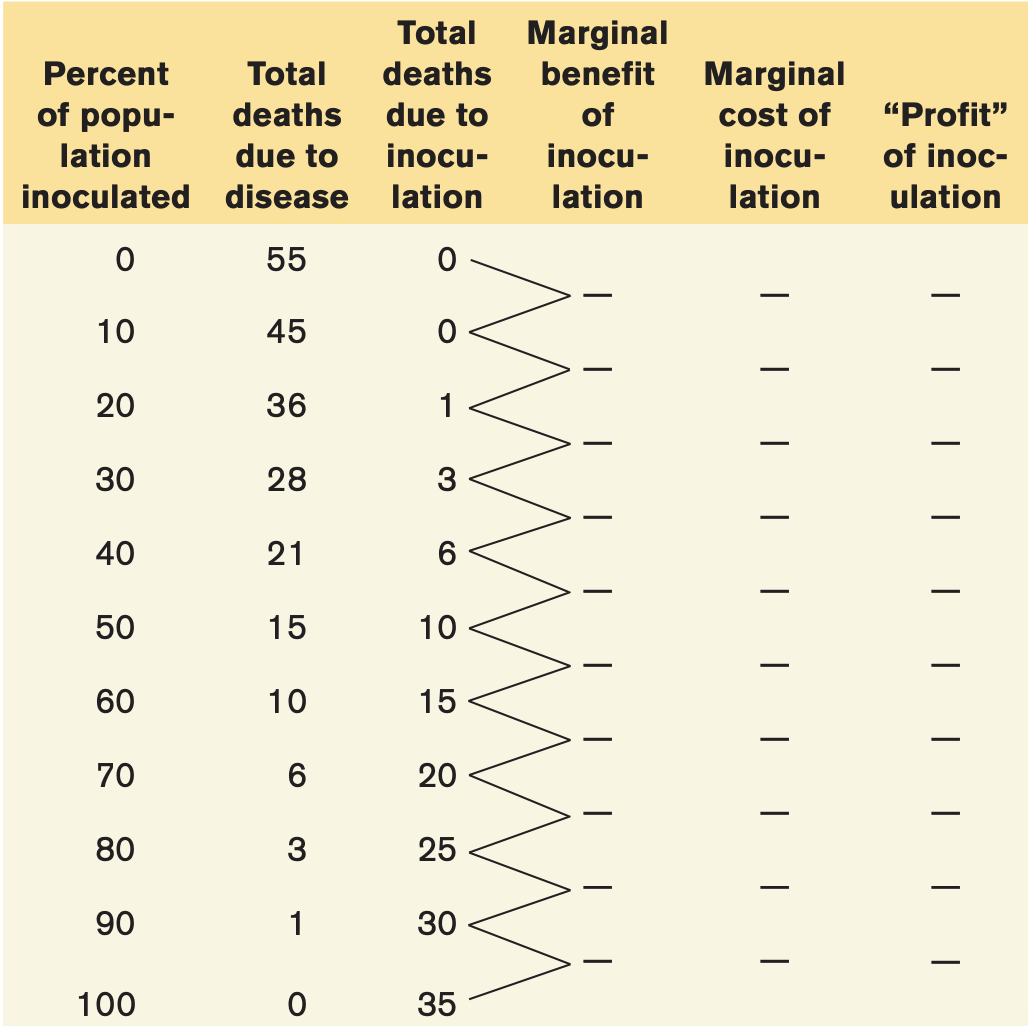
\includegraphics[width = 0.8\textwidth]{profit maximizing quantity problem}
	\end{center}
	
	\begin{enumerate}
	
	\item What are the interpretations of "marginal benefit" and "marginal cost" here? Calculate marginal benefit and marginal cost per each 10\% increase in the rate of inoculation. Write your answers in the table. 
	
	\item What proportion of the population should optimally be inoculated?
	
	\item What is the interpretation of "profit" here? Calculate the profit for all levels of inoculation.
	
	\end{enumerate}
	
\item The state of Maine has a very active lobster industry, which harvests lobsters during the summer months. During the rest of the year, lobsters can be obtained from other parts of the world but at a much higher price. Maine is also full of “lobster shacks,” roadside restaurants serving lobster dishes that are open only during the summer. Explain why it is optimal for lobster shacks to operate only during the summer.

\item Below are profit-maximizing rules for a competitive firm. Fill in the blank.

	\begin{enumerate}
	
	\item Find $Q$ at which $P = \underline{\phantom{MC}}$.
	
	\item If $P < \underline{\phantom{AVC}}$, shut down immediately and remain out of business.
	
	\item If $\underline{\phantom{AVC}} < P < \underline{\phantom{ATC}}$, operate in the short run but exit in the long run.
	
	\item If $\underline{\phantom{ATC}} < P$, stay in business and enjoy your profits!
	
	\end{enumerate}

\item Draw a short-run diagram showing a U-shaped average total cost curve, a U-shaped average variable cost curve, and a U-shaped marginal cost curve. On it, indicate the range of output and the range of price for which the following actions are optimal.

	\begin{enumerate}
	
	\item The firm shuts down immediately.
	
	\item The firm operates in the short run despite sustaining a loss.
	
	\item The firm operates while making a profit. 
	
	\end{enumerate}
	
\item Draw a short-run diagram showing a U-shaped average total cost curve, a U-shaped average variable cost curve, and a U-shaped marginal cost curve. On it, indicate the price at which the firm makes zero profit or loss.

\end{enumerate}

\end{document}